
\section{Unleashing the Power of Artificial Neural Networks (ANNs)}
In the previous chapters, we have discussed a key challenge encountered in neurons: the linearity of problems.
In some cases, problems are not linear and cannot be easily separated or solved using linear regression
techniques alone. To address this, we introduced the idea of using multiple neurons and now the time has
come to delve into building our first neural network from scratch. It's important to note that neural
networks have their own peculiarities and understanding linear algebra, including concepts such as matrix
construction and solving linear systems, will greatly aid in comprehending how these models truly function.
I highly recommend studying linear algebra to ensure a solid foundation for the upcoming explanations.\\

This approach of ANNs
is inspired by how our brain cells works. Our brain consists of billions of interconnected
neurons, and drawing from this concept, we can create
several artificial neurons and connect their outputs to inputs.
By adjusting the weights or parameters of the neural network, we can observe if it can produce valuable outputs.
In essence, we are attempting to mimic the functioning of the brain using artificial neural networks (ANNs).

\begin{figure}[H]
  \centering
  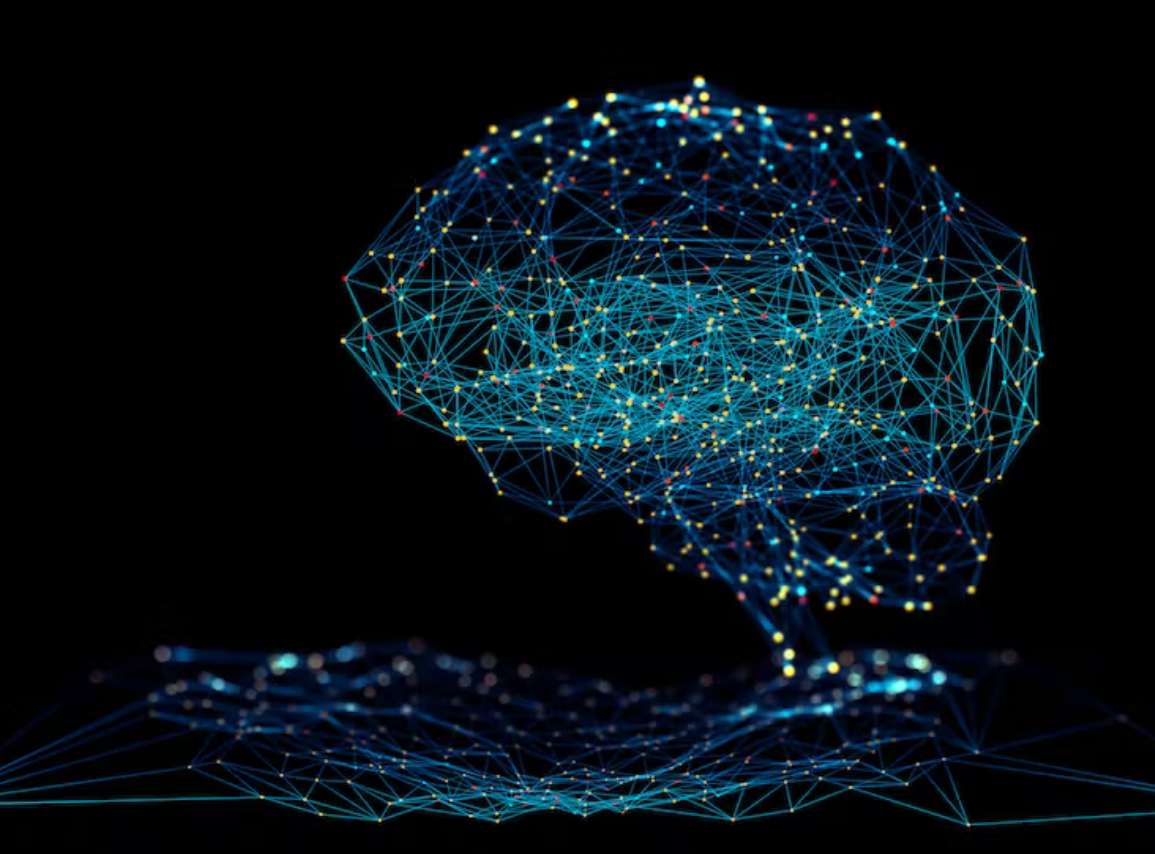
\includegraphics[scale = 0.3]{neural_networks.png}
  \caption{The brain cells}
\end{figure}
Next, let's examine the components of an Artificial
Neural Network to gain a better understanding of how they operate.
\subsection{Components of an Artificial Neural Network}
\begin{figure}[H]
  \centering
  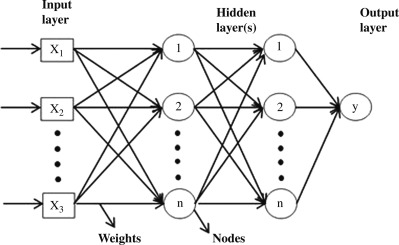
\includegraphics[scale = 1.3]{nerual_network.jpg}
  \caption{The neural network}
\end{figure}
\begin{itemize}
\item \textbf{Input Layer}: The input layer of a neural network may not always consist of artificial neurons.
  In certain cases, such as when combining multiple neural networks, the input can be sourced from the output
  of another neural network. However, in the context of a simple neural network, the input layer is represented
  by an array or vector that serves as the input data for the network.
  
\item \textbf{Hidden Layer}: The hidden layers of a neural network consist of groups of artificial neurons
  arranged vertically. Each hidden layer receives inputs and produces outputs. The term "hidden" refers to
  the fact that these layers are not directly observable from the network's input or output. The connections
  between the artificial neurons enable the flow of information and allow for complex computations to take
  place within the hidden layers.
  
\item \textbf{Output Layer}: The output layer, similar to the hidden layers, is composed of multiple neurons.
  In the previous image, only one node is shown for simplicity, but in reality, a neural network can have
  multiple output neurons, especially for classifying more complex patterns or performing multiple tasks
  simultaneously. The output layer receives the outputs from the hidden layers and performs the final
  computations to generate the desired output or prediction.
\end{itemize}
\subsection{The XOR Problem}
One of the limitations of the perceptron is its inability to solve the XOR logic gate problem, which is
not linearly separable. This means that a single neuron cannot accurately classify the XOR inputs.
I conducted an experiment to test this, and the results clearly show that the perceptron fails to converge
when trained on the XOR problem.
\begin{verbatim}
MSE: 0.250000
1, 1: 0.500000
0, 1: 0.500000
1, 0: 0.500000
0, 0: 0.500000
 Weights:    0.00000000       0.00000000       0.00000000    
\end{verbatim}
The mean squared error (MSE), which is our cost function, gives us an error of $0.25$, which is the lowest
achievable error. However, this result is quite peculiar because in computer architectures, an XOR logic
gate is typically implemented using other logic gates.
\begin{figure}[H]
  \centering
  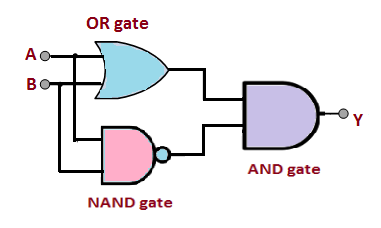
\includegraphics[scale = 1.0]{xor-equivalent-circuit.png}
  \caption{XOR equivalent circuit}
\end{figure}
As you can see, this illustrates the fundamental idea of neural networks: using multiple neurons to achieve
more complex and precise computations. The following diagram represents the XOR neural network,
which demonstrates the
power of combining neurons to solve non-linearly separable problems.


\begin{center}
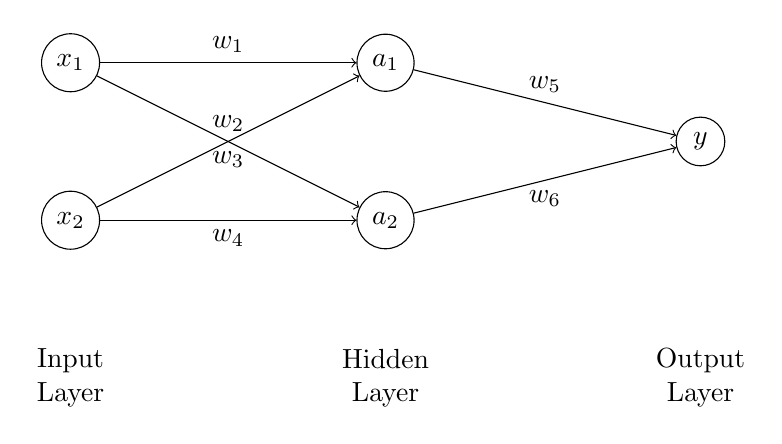
\begin{tikzpicture}[scale=2.0]
  % Input layer
  \node[circle, draw] (input1) at (0,0) {$x_1$};
  \node[circle, draw] (input2) at (0,-1) {$x_2$};

  % Hidden layer
  \node[circle, draw] (hidden1) at (2,0) {$a_1$};
  \node[circle, draw] (hidden2) at (2,-1) {$a_2$};

  % Output layer
  \node[circle, draw] (output) at (4, -0.5) {$y$};

  % Edges with weights
  \draw[->] (input1) -- node[midway, above] {$w_1$} (hidden1);
  \draw[->] (input2) -- node[midway, above] {$w_2$} (hidden1);
  \draw[->] (input1) -- node[midway, below] {$w_3$} (hidden2);
  \draw[->] (input2) -- node[midway, below] {$w_4$} (hidden2);
  \draw[->] (hidden1) -- node[midway, above] {$w_5$} (output);
  \draw[->] (hidden2) -- node[midway, below] {$w_6$} (output);

  % Labels
  \node[align = center] at (0, -2) {Input\\Layer};
  \node[align = center] at (2, -2) {Hidden\\Layer};
  \node[align = center] at (4, -2) {Output\\Layer};
\end{tikzpicture}
\end{center}

In total, this network architecture consists of three artificial neurons. Let's dive into the mathematical
calculations for these neurons. We can consider $a_1$ and $a_2$ as the result variables obtained from the
computations of those neurons. The mathematical expression utilizing the sigmoid function for these
computations is as follows.
\[
a_1 = \sigma(b_1 + x_1 \cdot w_1 + x_2 \cdot w_2)
\]
\[
a_2 = \sigma(b_2 + x_1 \cdot w_3 + x_2 \cdot w_4)
\]
If you study linear algebra, as mentioned at the beginning of this chapter, you will start noticing a pattern,
right? To be more precise, the expressions shown above exhibit a matrix multiplication. Let's take a closer
look: We can interpret our input vector $\vec{x} = \{x_1, x_2\}$ as a matrix $X$.
\[
X = \begin{bmatrix} x_1 \\ x_2 \end{bmatrix}
\]
And similarly, with our weights, in the previous chapter we saw our bias as part of the weight vector
$\vec{w} = \{b, w_2, \cdots, w_n\}$. However, for today's explanation, we will separate the bias
from the weights to simplify the equations and expressions.
\[
W_1 = \begin{bmatrix} w_1 & w_3 \\ w_2 & w_4 \end{bmatrix}
\quad
B_1 = \begin{bmatrix} b_1 \\ b_2 \end{bmatrix}
\]
And we can also consider $a_1$ and $a_2$ as elements of a result matrix. In matrix form, we can represent
them as:

\[
A_1 = \begin{bmatrix} a_1 \\ a_2 \end{bmatrix}
\]

And essentially, with these matrices, we can abstract the above computations as simple matrix
multiplications followed by passing the result through an activation function. Take a look:
\[
A_1^T = \sigma(X^T \cdot W_1 + B_1^T) = \begin{bmatrix} a_1 & a_2 \end{bmatrix}
\]

when we use $X^T$, it refers to the transpose matrix of $X$, which means rearranging the components of the
matrix into a different order. This allows us to perform operations such as matrix multiplication
between $X^T$ and another matrix, taking into account the rearranged structure.
\[
X = \begin{bmatrix} x_1 \\ x_2 \end{bmatrix}
\]
\[
X^T = \begin{bmatrix} x_1 & x_2 \end{bmatrix}
\]
And this is not the only approach to performing these computations. Another way is to consider the transpose
of $W$ instead of $X$. Both approaches yield the same results. I mention this to avoid confusion if you come
across different explanations while learning about these concepts elsewhere.
\[
A_1 = \sigma(W_1^T \cdot X + B_1) = \begin{bmatrix} a_1 \\ a_2 \end{bmatrix}
\quad \quad A_1 = \sigma(\begin{bmatrix} w_1 & w_2 \\ w_3 & w_4 \end{bmatrix} \cdot
\begin{bmatrix} x_1 \\ x_2 \end{bmatrix} + \begin{bmatrix} b_1 \\ b_2 \end{bmatrix}) =
\begin{bmatrix} a_1 \\ a_2 \end{bmatrix}
\]
It is important to note that the order of matrix multiplication determines the structure of the resulting
matrix. In the context of neural networks, this concept becomes significant. After obtaining the matrix $H_1$
from the previous computations, it is used as input for the next layer. This process of passing outputs from
one layer to another forms the basis of the feedforward operation in a neural network. As you can see, it is
a sequential flow of matrix operations.
\[
W_2 = \begin{bmatrix} w_5 \\ w_6 \end{bmatrix} \quad
Y = \sigma(W_2^T\cdot A_1 + B_2) = \begin{bmatrix} y \end{bmatrix} = y
\]

At the end, a simple number can be thought of as a matrix with a single component, represented as $Y = [y] = y$.
This approach allows us to treat scalar values as matrices, ensuring consistency and compatibility with matrix
operations in neural networks. As you can see, it is not overly complicated from a matrix perspective.
\subsection{Understanding Feedforward in Artificial Neural Networks}
Feedforward is a commonly used term in artificial intelligence, referring to the process of taking an input and
passing it through the layers of complexity to obtain an output. By abstracting the artificial neuron layers
to matrices, we can simplify the computation of each layer. In essence, we can think of this process as follows:
\[
A_l = f(W_l^T \cdot A_{l - 1} + B_l) = \begin{bmatrix} a_{1}^l \\ \vdots \\ a_{n}^l \end{bmatrix}
\]
In the equation, $A_{l-1}$ represents the output from the previous layer. We observe that $A_{l-1}$ has the same
number of rows as the number of columns in $W_l^T$. This is denoted by the outputs $a_{1}^l, \ldots, a_{n}^l$,
where $l$ represents the current layer. This notation enables us to distinguish between the various outputs
$a$ across the network. Additionally, $W_l$ and $B_l$ correspond to the weight matrix and bias vector of the
current layer, respectively, while $f$ represents the activation function.
\[
W_l = \begin{bmatrix} w_{1, 1}^l & w_{1, 2}^l & \cdots & w_{1, n}^l \\
  w_{2, 1}^l & w_{2, 2}^l & \cdots & w_{2, n}^l \\
  \vdots & \vdots & \cdots & \vdots \\
  w_{m, 1}^l & w_{m, 2}^l & \cdots & w_{m, n}^l
\end{bmatrix}
\quad\quad B_l = \begin{bmatrix} b_{1}^l \\ b_{2}^l \\ \vdots \\ b_{n}^l \end{bmatrix}
\]
In this context, $n$ refers to the number of neurons in the current layer, and $m$ represents
the number of weights associated with each neuron or the number of neurons in the previous layer.
The subscript $l$ indicates the current layer. Additionally, the transpose of the weight matrix can be
represented as follows:
\[
W_l^T = \begin{bmatrix} w_{1, 1}^l & w_{2, 1}^l & \cdots & w_{m, 1}^l \\
  w_{1, 2}^l & w_{2, 2}^l & \cdots & w_{m, 2}^l \\
  \vdots & \vdots & \cdots & \vdots \\
  w_{1, n}^l & w_{2, n}^l & \cdots & w_{m, n}^l
\end{bmatrix}
\]
At the end, the structure of the initial $W_l$ can be simplified to avoid complexity. There isn't just one
way to approach these computations; it depends on the perspective you choose and what you consider to be the
most optimal method.
\[
W_l = \begin{bmatrix} w_{1, 1}^l & w_{1, 2}^l & \cdots & w_{1, m}^l \\
  w_{2, 1}^l & w_{2, 2}^l & \cdots & w_{2, m}^l \\
  \vdots & \vdots & \cdots & \vdots \\
  w_{n, 1}^l & w_{n, 2}^l & \cdots & w_{n, m}^l
\end{bmatrix}
\]

\[
A_l = f(W_l \cdot A_{l - 1} + B_l) = \begin{bmatrix} a_{1}^l \\ \vdots \\ a_{n}^l \end{bmatrix}
\]

Just keep in mind the variables $m$, which represent the number of weights or the number of neurons from the
previous layer, and the variable $n$, which refers to the number of neurons in the current layer.
When discussing the algorithmic process, we repeat this computation for all $l$ layers. So, you can think of
the first layer as follows:
\[
A_1 = f(W_1 \cdot X + B_1) = \begin{bmatrix} a_{1}^1 \\ \vdots \\ a_{n}^1 \end{bmatrix}
\]
Then, we can consider the last layer as the output layer $k$ and it should be something as follows:
\[
Y = A_k =  f(W_k \cdot A_{k - 1} + B_k) 
= \begin{bmatrix} a_{1}^k \\ \vdots \\ a_{n}^k \end{bmatrix}
= \begin{bmatrix} y_{1} \\ \vdots \\ y_{n} \end{bmatrix}
\]
Where $k$ is the last layer from this system.
I understand that there is a lot of notation involved, but it is crucial to have a clear understanding of all
the variables and their meanings. The feedforward process can be seen as a composition of multiple functions,
where each layer's output serves as the input for the next layer. It is important to ensure that you can
comprehend this expression and its implications.
\[
Y = f(W_k \cdot f(
W_{k - 1} \cdot f(\cdots f(W_{1} \cdot X + B_1) \cdots) + B_{k - 1}
) + B_k) = \begin{bmatrix} y_1 \\ \vdots \\ y_{r} \end{bmatrix}
\quad \quad | \quad \quad X = \begin{bmatrix} x_1 \\ \vdots \\ x_{d} \end{bmatrix}
\]

Rather than treating it as a basic function, it is crucial to recognize that an artificial
neural network operates
as a nonlinear system. Unlike the perceptron, which processes individual inputs, a neural network receives
a column vector or matrix $X$ and generates an output column vector or matrix $Y$.

\[
\mathcal{N}: \quad \mathbb{R}^d \quad  \rightarrow \quad \mathbb{R}^r \quad | \quad d,r \in \mathbb{N} 
\]
Where $\mathcal{N}$ represent the artificial neural network.
Mathematically speaking, artificial neural networks can be understood as linear transformations or mappings.

\subsection{Intuition Behind Neural Networks}
The underlying concept behind these expressions and neural networks is that each layer creates an
abstraction of the input data. Whether it's detecting patterns for linear separability or regression,
each layer captures and quantifies the presence of these patterns. This information is then passed on
to the next layer of neurons, and this process continues until reaching the output layer, which ultimately
makes a decision or classification.

To illustrate this concept, consider a child learning to identify clocks. At the initial stage, the child
recognizes that a clock is a circular object, representing the first level of abstraction. As the child
progresses, they discover that clocks have numbers and an arrow, representing a second layer of abstraction.
Eventually in the last layer, the child grasps the concept of telling time, which emerges from these layers
of abstractions. This is analogous to how a neural network understands and learns.

by each individual neuron within these layers remains somewhat mysterious due to the complexity of the
underlying mathematical derivatives, which we will discuss in the next section. The key point here is that
the hidden layers operate at a highly abstract level, and through a process of convergence, the network as a
whole learns to perform seemingly magical computations. This is the unleashing power of neural networks,
where these parameters or weights enable the network to abstract and classify more complex concepts and ideas.

\section{How to train an Artificial Neural Network?}
As I mentioned earlier, training a neural network is not an easy task. In fact, the concept of
ANNs is not new and dates back to the 1960s. However, during that time, the main challenges were
related to computing power and the lack of understanding of effective training methods.

Let's break it down step by step. First, we need to define a cost function that quantifies the error of
our model.
However, this task can be somewhat challenging starting with
the fact that a neural network can have multiple outputs.

\[
Y = \begin{bmatrix} y_1 \\ \vdots \\ y_n \end{bmatrix}
\]

Therefore, for each output generated by our neural network, there should be a corresponding desired output.
\[
Y_t = \begin{bmatrix} y_{1}^t \\ \vdots \\ y_{n}^t \end{bmatrix}
\]

Here, $t$ represents the current training example for each input matrix $X_t$.
From this, we can infer that for each $y_{i}^t$, we can calculate an error measurement.
\[
E =
\begin{bmatrix}
  \frac{1}{N} \cdot \sum_{t = 1}^{N}(y^t_{1} - \overset{\sim}{y_{1}^t})^2 \\ \vdots \\
  \frac{1}{N} \cdot \sum_{t = 1}^{N}(y^t_{n} - \overset{\sim}{y_{n}^t})^2
\end{bmatrix}
\]

Here, $\overset{\sim}{y_{1}^t}$ represents the predicted output from the neural network. We can
interpret the matrix or vector of errors by summing up all the individual errors, with $N$ being the
size of the dataset $\mathbb{D}$. Since this matrix has only one column, we can simplify the calculation
by using a single summation; this is called the \textbf{grand sum} in the field of mathematics.
This expression, often referred to as
the cost function or loss function, provides a measure of the error generated by the neural network.

\[
C = \sum_{i = 1}^{n} E_{i, 1}
\]

Indeed, all the weights in our neural network have an impact on the error expression. This complexity is
what makes training a neural network challenging. It becomes difficult to find an expression that guides
us in updating the weights effectively. Just imagine the task of deriving an expression to update the
weights—it's quite daunting.
\[
\frac{\partial C}{\partial w_{i, j}^{(l)}} = ?
\]

However, it is important to remember that the output $Y$ of a neural network is a composition of numerous
activation functions. This complexity makes it extremely challenging to derive mathematical expressions for
computing the partial derivatives with respect to each weight. It can feel overwhelming due to the sheer number
of computations involved.

\[
Y = f(W_k \cdot f(
W_{k - 1} \cdot f(\cdots f(W_{1} \cdot X + B_1) \cdots) + B_{k - 1}
) + B_k) = \begin{bmatrix} y_1 \\ \vdots \\ y_{n} \end{bmatrix}
\]

For small neural networks, it is possible to derive general formulas for updating each weight using the
chain rule. However, this approach becomes impractical and non-scalable for larger networks due to the
complexities involved in programming and implementation. As an alternative, we can use finite differences
to approximate the derivatives. Although this introduces some bias in the precision of our calculations,
the main challenge lies in the computational cost. As the neural network grows in size, both in terms of
layers and weights, the time required to compute the approximate derivatives increases exponentially.
Despite this drawback, using finite differences allows us to address the problem by brute-forcing each
individual derivative.\\

\subsection{Brute forcing learning algorithm}
The approach of finite differences involves choosing a small value for $h > 0$ and adopting a
computational method. In this scenario, we consider our cost function as $f$ and $x_i$ as the weight
for which we want to approximate its rate of change with respect to $C$.
\[
\frac{\partial (f(\vec{x}))}{\partial x_i} \approx \frac{f(x_1, \cdots, x_i + h, \cdots, x_n) -
  f(x_1, \cdots, x_i, \cdots, x_n)}{h}
\]
Implementing this approach requires computing the actual cost $C$ using the current weights,
which in turn necessitates calculating all the outputs for the given dataset.
\[
C = \sum_{i = 1}^{n} E_{i, 1}
\quad | \quad
E =
\begin{bmatrix}
  \frac{1}{N} \cdot \sum_{t = 1}^{N}(y^t_{1} - \overset{\sim}{y_{1}^t})^2 \\ \vdots \\
  \frac{1}{N} \cdot \sum_{t = 1}^{N}(y^t_{n} - \overset{\sim}{y_{n}^t})^2
\end{bmatrix}
\quad | \quad \mathcal{N}: X_t \rightarrow Y_t
\quad \forall X_t \in \mathbb{D}
\]
In this case, $\mathcal{N}$ represents our neural network, which maps input $X_t$ to output $Y_t$. Therefore,
to obtain our desired cost function, we must compute all the outputs for the entire dataset
$\mathbb{D}$. Once we have the actual cost, we can proceed to modify the specific weight $w_{i, j}^l$
using a small value of $h$.
\[
w_{i, j}^{(l)} + h = \overset{\sim}{w_{i, j}^{(l)}}
\]
After making a small change to the network, we need to compute the modified version of $C$,
denoted as $\overset{\sim}{C}$. This implies that we must recompute all the outputs for the entire dataset again.
\[
\overset{\sim}{C}= \sum_{i = 1}^{n} E_{i, 1}
\quad | \quad E =
\begin{bmatrix}
  \frac{1}{N} \cdot \sum_{t = 1}^{N}(y^t_{1} - \overset{\sim}{y_{1}^t})^2 \\ \vdots \\
  \frac{1}{N} \cdot \sum_{t = 1}^{N}(y^t_{n} - \overset{\sim}{y_{n}^t})^2
\end{bmatrix}\quad | \quad \mathcal{N}: X_t \rightarrow Y_t
\quad \forall (X_t,Y_t) \in \mathbb{D}
\]

I don't know about you, but computing matrix multiplications can be quite time-consuming.
After going through all these calculations, we finally obtain an approximation of the rate of change.

\[
\frac{\partial C}{\partial w_{i, j}^{(l)}} \approx \frac{\overset{\sim}{C} - C}{h}
\]

Yes, we have finally completed the process. Now, we just need to repeat this entire process for each
weight $w_{i, j}^{(l)}$ within the neuron, then for each layer $l$ until you reach $k$ layer. However,
this approach is highly inefficient and computationally demanding. In fact, back in the 1960s, with the
limited computing power available, it was not feasible to perform these calculations. Even today, with
more powerful computers, performing deep learning tasks using this algorithm on a regular desktop computer
is simply impractical.\\

Throughout this chapter, we have not delved into any deep learning ANNs.
However, in the next chapter,
we will explore how to address this issue and optimize the learning algorithm for ANNs.
We will introduce the Back Propagation algorithm, which builds upon the fundamental principles of
gradient descent and provides a solution for adjusting the weights without relying on brute force methods.

\section{The Convergence Proof of ANNs}
Understanding the convergence proof of Artificial Neural Networks (ANNs) can be quite challenging, and it
has been a serious struggle for me. I lack the abilities to grasp the intricacies of the convergence proof
fully. However, we can still develop an idea of it by considering the concept of gradient descent.
Essentially, gradient descent plays a crucial role in fitting the weights of the neural network.

\[
\frac{\partial C}{\partial w_{i, j}^{(l)}}
\]

Remember that with gradient descent, we have a clear path to move and adjust each of the $w_{i, j}^{(l)}$ in the
system. You only need to arrive at a good measurement of the error from the model; that's the key. By using
gradient descent, the model should converge.

\section{Coding Our First Neural Network}
With these components in place, including the essential matrix component
I recommend you to write a class or structure to track the values from the matrix, you can construct a functional
neural network with ease. The layer component is optional but can build it to enhance the organization of
your codebase.
Additionally, make sure to include the cost functions to evaluate and optimize your model effectively.

\begin{enumerate}
\item Matrix
\item Activation Function
\item Layer \textbf{(Not necessary)}
\item Cost Functions
\item Model \textbf{(ANNs model)}
\end{enumerate}

\subsection{The matrix component}
The matrix component must have the basic operations like addition, subtraction, multiplication.
\begin{verbatim}
structure Matrix:
    // Private variables
    rows: integer      // Number of rows in the matrix
    cols: integer      // Number of columns in the matrix
    data: 2D array    // 2D array to store the matrix elements

    // Constructor to initialize the matrix
    function initialize(rows, cols):
        this.rows = rows
        this.cols = cols
        this.data = create a new 2D array with dimensions (rows, cols)

    // Function to access a specific element in the matrix
    function operator()(row, col):
        return data[row][col]
\end{verbatim}

\subsubsection{Matrix addition and substraction}
The addition and subtraction algorithms are not hard to build; this is a pseudo-code.
\begin{verbatim}
# Function to perform matrix addition
function matrix_add(matrix1, matrix2):
    if dimensions of matrix1 and matrix2 are not the same:
        return "Error: Incompatible matrices"
    
    rows = number of rows in matrix1
    cols = number of columns in matrix1
    
    result_matrix = create a new matrix with dimensions (rows, cols)
    
    for i from 0 to rows:
        for j from 0 to cols:
            result_matrix[i][j] = matrix1[i][j] + matrix2[i][j]
            
    return result_matrix

# Function to perform matrix subtraction
function matrix_subtract(matrix1, matrix2):
    if dimensions of matrix1 and matrix2 are not the same:
        return "Error: Incompatible matrices"
    
    rows = number of rows in matrix1
    cols = number of columns in matrix1
    
    result_matrix = create a new matrix with dimensions (rows, cols)
    
    for i from 0 to rows:
        for j from 0 to cols:
            result_matrix[i][j] = matrix1[i][j] - matrix2[i][j]
            
    return result_matrix
\end{verbatim}
\subsubsection{Matrix multiplication}
Additionally, the matrix multiplication algorithm is not hard to implement. The standard algorithm works well,
but I recommend investigating the \textbf{Strassen algorithm}, which is much faster and scalable for large
neural networks with big layers of neurons, for the moment you can code this algorithm.
\begin{verbatim}
# Function to perform matrix multiplication
function matrix_multiply(matrix1, matrix2):
    if number of columns in matrix1 is not equal to number of rows in matrix2:
        return "Error: Incompatible matrices"
    
    rows_in_matrix1 = number of rows in matrix1
    cols_in_matrix1 = number of columns in matrix1
    cols_in_matrix2 = number of columns in matrix2
    
    result_matrix = create a new matrix with dimensions (rows_in_matrix1, cols_in_matrix2)
    
    for i from 0 to rows_in_matrix1:
        for j from 0 to cols_in_matrix2:
            dot_product = 0
            for k from 0 to cols_in_matrix1:
                dot_product += matrix1[i][k] * matrix2[k][j]
            result_matrix[i][j] = dot_product
            
    return result_matrix  
\end{verbatim}

\subsection{The activation functions}
Then the activation functions should run over the matrix components. For that reason, once again,
I recommend that you code the matrix as a structure or class to keep track of the values from the matrix.
\subsubsection{The activation function sigmoid:}
This is the classical activation function that you are already familiar with. I will now code it to operate
over the matrix.
\begin{verbatim}
function sigmoid(matrix m):
    for i from 0 to rows of m:
        for j from 0 to columns of m:
            m(i, j) = 1.0 / (1 + exp(-m(i, j)))
    return m
\end{verbatim}
\subsubsection{The activation function relu:}
This is the most commonly used activation function for ANNs, and once again, we will apply it to the matrix.
\begin{verbatim}
function sigmoid(matrix m):
    for i from 0 to rows of m:
        for j from 0 to columns of m:
            m(i, j) = 1.0 / (1 + exp(-m(i, j)))
    return m
\end{verbatim}

\subsection{The layer component}
While the layer component is not necessary, I recommend you to code it because it will make your codebase
more organized. This component will simply store two matrices: the weights and biases. It will also include a
function called "feedforward" where we will perform the matrix multiplication of the weights, addition of the
biases, and apply the activation function.
\begin{verbatim}
structure Layer:
    // Private variables
    weights: Matrix    // Matrix to store the weights
    biases: Matrix     // Matrix to store the biases
    activation_function: function pointer   // Pointer to the selected user activation function

    // Constructor to initialize the layer with given weights, biases, and activation function
    function initialize(weights, biases, activation_func):
        this.weights = weights
        this.biases = biases
        this.activation_function = activation_func

    // Function to perform feedforward operation
    function feedforward(input_matrix):
        // Perform matrix multiplication of weights and input matrix
        multiplied_matrix = matrix_multiply(weights, input_matrix)

        // Add biases to the multiplied matrix
        output_matrix = matrix_add(multiplied_matrix, biases)

        // Apply the user-selected activation function
        activated_output = activation_function(output_matrix)

        return activated_output
\end{verbatim}

\subsection{The cost functions}
With the invention of neural networks, various cost functions are available. However, for the moment, we
will use the MSE (Mean Squared Error) function and apply it to work with a matrix data type. Remember the
"grand sum" function, which will sum all the components from the result matrix or vector.
\begin{verbatim}
function grand_sum(matrix):
    sum = 0.0
    for i from 0 to rows of matrix:
        for j from 0 to columns of matrix:
            sum += matrix(i, j)
    return sum

function mean_squared_error(neural_network, input_data, output_data, training_size):
    cost = 0.0

    for i from 0 to training_size:
        predicted_output = neural_network.feedforward(input_data[i])
        error = matrix_subtract(output_data[i], predicted_output)
        squared_error = matrix_multiply(error, error)
        cost += grand_sum(squared_error)

    return cost
\end{verbatim}
\subsection{The model component}
The model component must be a component where you initialize it with an architecture. You can define the
architecture using an array, similar to how TensorFlow does it. In my case, I decided to define it with an
array like this:
\begin{verbatim}
 nn_arch arch[] = [2, 2, 1] // [input, hidden, ..., hidden, output]
\end{verbatim}
This array is then received by the neural network model to define its architecture.
\begin{verbatim}
structure NeuralNetwork:
    // Private variables
    architecture: array    // Array to store the architecture of the model
    layers: array          // Array to store the layers of the model

    // Constructor to initialize the model with the given architecture
    function initialize(architecture_array):
        this.architecture = architecture_array
        this.layers = create a new empty array

        // Create the layers based on the architecture
        for i from 0 to size of architecture - 1:
            input_size = architecture[i]
            output_size = architecture[i + 1]

            // Initialize the layer with random weights and biases
            layer = Layer(initialize_random_weights(input_size, output_size), 
                          initialize_random_biases(output_size))

            // Add the layer to the layers array
            layers.add(layer)

    // Function to perform the forward pass of the neural network
    function feedforward(input_data):
        output = input_data

        // Iterate through all layers and perform feedforward
        for each layer in layers:
            output = layer.feedforward(output)

        return output
\end{verbatim}

\subsubsection{The training algorihtm code}
As I mentioned previously, we are not going to use the backpropagation algorithm. Instead, we will use
finite differences. Keep in mind that this method is computationally expensive, and you will see why.
\begin{verbatim}
function fit_neural_network(input, output, train_size, learning_rate, num_epochs):
    while num_epochs > 0:
        h = 0.00001
        
        for l from 0 to number of layers - 1:
            for i from 0 to number of rows in weights of layer[l]:
                for j from 0 to number of columns in weights of layer[l]:
                    c = calculate_mse_loss(neural_network, input, output, train_size)
                    neural_network.layers[l].weights(i, j) += h
                    dc = mean_squared_error(neural_network, input, output, train_size)
                    neural_network.layers[l].weights(i, j) -= h
                    neural_network.layers[l].weights(i, j) -= learning_rate
                                                            * (dc - c) / h
                
            for i from 0 to number of rows in biases of layer[l]:
                for j from 0 to number of columns in biases of layer[l]:
                    c = calculate_mse_loss(neural_network, input, output, train_size)
                    neural_network.layers[l].biases(i, j) += h
                    dc = mean_squared_error(neural_network, input, output, train_size)
                    neural_network.layers[l].biases(i, j) -= h
                    neural_network.layers[l].biases(i, j) -= learning_rate
                                                           * (dc - c) / h
        
        num_epochs -= 1
\end{verbatim}
As you can see, this method is computationally expensive because for each weight $w_{i, j}^{(l)}$, we
need to compute the cost, add a small difference to that weight, and then recompute the cost of the model.
Now, imagine having a massive neural network; this process becomes even more computationally intensive.
However, for our purpose, it still works despite its cost. If you want to optimize your model, what I
recommend is to compute the cost function $c$ once for each layer and then compute $dc$ for each weight. This
approach could reduce the computational burden to some extent, though it might slightly affect the precision
of your model.

\section{Examples}
For my code examples, I decided to use \href{https://www.netlib.org/blas/}{BLAS}. You can find these examples
at this repository: \href{https://github.com/alecksandr26/fortran-ml/tree/main/examples}{examples}. Please
feel free to review these examples while you continue reading this section.

\subsection{Example neural network code in fortran}
To build a neural network, the codebase cannot be put in just one file. You can find the code shown in these
notes through the following link:
\href{https://github.com/alecksandr26/fortran-ml/tree/main/src}{src}.



